\section{Items and Monsters}

Items and monsters works in many way the same even though monsters also share some common traits with the player class.
Both monsters and items has a title/name, description etc.

\begin{figure}[ht!]
	\centering
	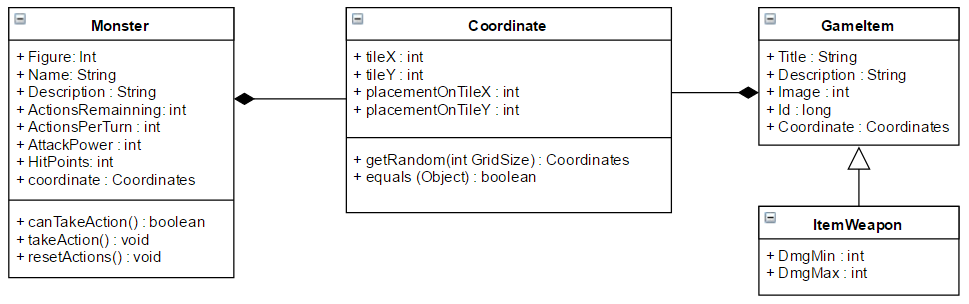
\includegraphics[width=130mm]{images/itemsAndMonstersDiagram.png}
	\caption{Class diagram for monsters and items - Constructors, Getters and Setters has been left out}
	\label{fig:itemsAndMonstersDiagram}
\end{figure}

In the first version of the game neither Monster nor GameItem had Coordinate as a property. Instead it was a list of tuples. The tuples consisted of a monster or game item and a coordinate. It however turned out to be quite difficult to work with, since one had to loop through the list of tuples quite a lot just to get the right monster. It also made it difficult to update the game state, due to these looping and parsing of tuples in methods instead of the monster or game item object. Therefore we changed it to the design shown on figure \ref{fig:itemsAndMonstersDiagram}. When a player picks up an item the coordinate property of that item is then set to null. \\

\subsection{Factories}
Both items and monsters are created via a factory. When creating a monster or item, the gameview request a random item or monster. Currently items are totally randomized and monsters are separated into class'. See "Future Improvements" for more information about future ideas and improvements.
